
\subsection{Classical solution}
There are several classical methods of integer factorization. Some of the notable methods are
\subsubsection{Brute force}
To factor an integer $I$, one could run an algorithm from 2 to $I$ to check if any of them divides $I$ exactly. The ones that divide exactly or numbers that are not co-prime with $I$ $(\neg x \phi I)$ are factors. This algorithm would take $O(N) steps = O(2^w)$ steps where $w= \log_2 I$ is the length of I.

With a little analysis, we could prove that any factor of n would be less than the square root of $ I(P<\sqrt{ I})$. Hence, the loop could be reduced to $\sqrt{ I}$ times. It has $O(\sqrt{ I}) = O(2^{\frac{w}{2}})$ complexity which is exponential.

\subsubsection{GNFS - General Number Field Sieve}
It is the best known classical algorithm for prime number factorization developed by John Pollard in 1996. It factorizes large integer into its factor in a super polynomial or sub-exponential time. The asymptomatic complexity of GNFS is $ O(e^{{(\log I)}^{\frac{1}{3}} (\log(\log I))^{\frac{2}{3}}})$ = $O(e^{w^{\frac{1}{3}} (\log w)^{\frac{2}{3}}})$ where I is number to be factored and $w= \log I$\cite{hamdi_2014}



\section{Shor's Algorithm} 
Shor's Algorithm is a quantum algorithm for composite integer factorization with polynomial time complexity.\cite{shor1994} This algorithm could factor a number I that has a product of two primes : P and Q such that $I=P.Q$ with $\mathcal{O}(log^3(I))$ complexity for large I. Shor developed this algorithm in 1994. The paper is considered a "landmark paper " in quantum computing.\cite{Hidary} (Hidary, 2019) This algorithm sets a significant practical milestone that sparked the interest of a lot of physicists, computer scientists, and mathematicians in the field.

Integer factorization is a problem that is considered an NP (Non-polynomial) class problem in classical computing for its exponentially increasing complexity. Shor's Algorithm exploits parallelism, interference, and other properties of a quantum computer to get a quantum speed up to its classical counterparts.

The following graph shows the difference in the complexity of Different algorithms with Shor's algorithm.
\begin{figure}[H]
  \centering
  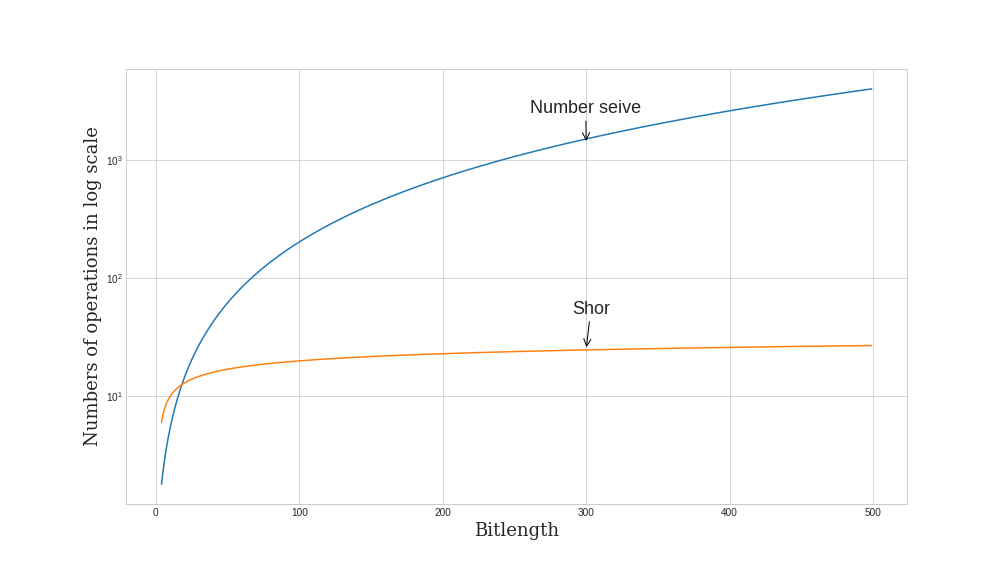
\includegraphics[width = \linewidth]{figures/numberseive_vs_shor.png}
      \caption{Figure showing complexity of Shor's algorithm and number field seive }
  \label{fig: complexity_comparision}
\end{figure}

 
\section{Workings of Shor's Algorithm}
Let $I \in \; \mathbb{Z}$ be a composite number, the goal is to find a prime number $p$ such that p exactly divides I or $p|I$. \\
 we divide  I into three categories for the study:
 \renewcommand{\labelenumi}{\Roman{enumi}}
 \begin{enumerate}
     \item $I$ is even, $I= 2z$, $z \in \mathbb{Z}^+$
     \item $I$ is power of a prime(p), $m = p^k$, $k \in \mathbb{Z}^+$
     \item $I$ is odd and is not power of prime
 \end{enumerate}
\paragraph{Case I \\} 
For an even $I$, it is easy to find the prime factor, that is, 2. The next prime factor can be determined using the found factor.
\paragraph{Case II \\}
Case II is also a classically polynomial problem. For $m = p^k$, $k \in \mathbb{Z}^+$, the exponent $k$ satisfies $ logI > k$ since $I > p$ and  $p = \lfloor \sqrt[k]{I} \rfloor$. \\
Iterating $j$ from 2 to $log I$ on $p_j = \lfloor \sqrt[j]{I} \rfloor$ would give  $(log I- 1)$ values for $p_j$. The $p_j$'s is checked if $(p_j)^j = I$. The smallest $p_j$ to satisfy the condition is the prime factor.
\paragraph{Case III \\}
Shor's algorithm only solves the factoring problem for the third case. The exponentially large classical complexity for the factoring problem, we discussed earlier arise due to case III. We assume I to be odd and is not the power of prime for the rest of the study.
\section{Shor's algorithm: Number Theory Approach}
We assume Case III: $I$ is not even and is not the power of the prime
 \renewcommand{\labelenumi}{\arabic{enumi}}
\begin{enumerate}
    \item Choose a random number : $ 1 < x < I $
    \item If $GCD(x , I ) \neq 1,$ then factor $= GCD(x, I)$ where $GCD$  = greatest common divisor
    \item If $GCD(x, I) = 1,$ find period or order '$a$' of a function
    $f(r) = x^r mod     , r\in \mathbb{Z}(I)$
    \item If period: $a$ is odd or $x^\frac{a}{2} \equiv -1(modI)$, we restart the algorithm from step 1.
    \item If $a$ is even and $x^\frac{a}{2} \equiv 1(modI)$ then, factors of $I$ are: $p= GCD(x^
    \frac{a}{2} + 1, I)$ and $q = GCD(x^\frac{a}{2} - 1, I)$.
\end{enumerate}

\subsubsection{Random selection of x}
    If the GCD of randomly selected $x$ and $I$ is not 1, it means $x$ and $I$ share a factor and the GCD gives the factor of $N$. If $GCD(x, I) = 1$, it means $x$ and $I$ are co-prime with each other.
\subsubsection{Find order of modular exponential function}
    Since $x$ and $I$ are co-prime, by theorem (\ref{th: exist_order_z_N}), order or period of function $x^r mod I$ exist. The process of order finding is the most difficult task in Shor’s algorithm. The complexity of order finding grows exponentially as the bit-length of $I$. Figure(\ref{fig: period_finding_complexity})and (\ref{fig: period_finding_complexity_time}) shows the classical growth of complexity of the task.
    \begin{figure}[ht]
    \centering
    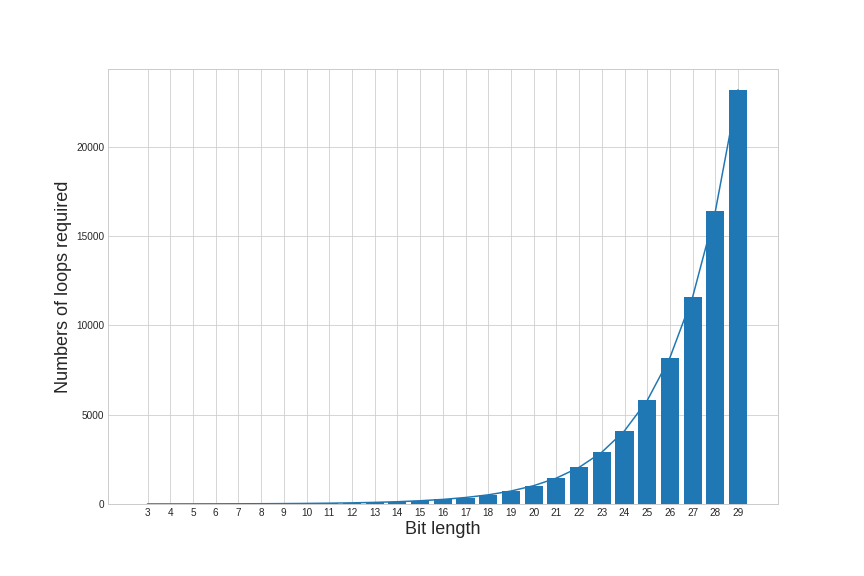
\includegraphics[width=\linewidth]{figures/nuum_loops_vs_bits.png}
    \caption{Graph of bit-length versus maximum number of loops needed to find period for the integer}
    \label{fig: period_finding_complexity}
    \end{figure}
     \begin{figure}[ht]
    \centering
    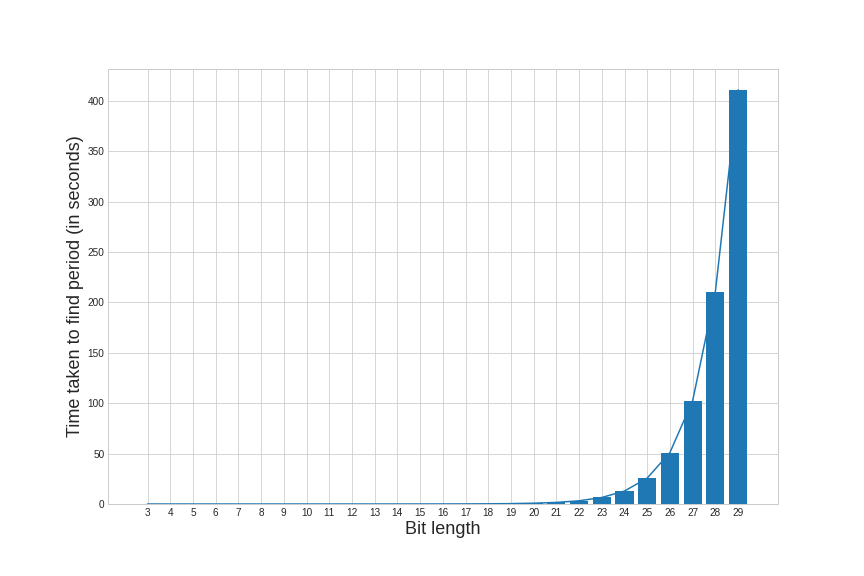
\includegraphics[width=\linewidth]{figures/time_period_vs_bits.png}
    \caption{Graph of bit-length versus time required to find period for the integer}
    \label{fig: period_finding_complexity_time}
    \end{figure}
We will discuss the process of the order finding in polynomial time using Quantum Computer later in the study.
\subsubsection{Determine factors using order 'a'}

 
\begin{theorem}
    Suppose $I$ is a composite number and $0<x< I$ ; $x \in \mathbb{Z}$ such that function $f(r)=x^r mod I$ has even period, a and $x^a \not \equiv -1 mod I$, then $I$ has non trivial factors given by $GCD(x^{\frac{a}{2}} -1, I ) $ and $GCD(x^{\frac{a}{2}} +1, I )$ \cite{Nielsen2002}
    \label{th:factors_GCD_pm}
\end{theorem}
\begin{proof}
    Since a is period of function: $f(r)=x^r $mod I, $x^a \equiv 1$ mod $I$ 
    \begin{center}
         $\Rightarrow (x^{\frac{a}{2}}-1) (x^{\frac{a}{2}} +1)\equiv 0$ mod $I$
    \end{center}
    Also, we know, $(x^{\frac{a}{2}} \not \equiv 1$ mod $I$) or $(x^{\frac{a}{2}}-1) \not\equiv 0$ mod $I$) as it contradicts that $a$ is order of function. Also, by definition, we have, $(x^{\frac{a}{2}} +1) \not\equiv 0$ mod $I$. 
    \\Hence we could find the non-trivial factors that are: $GCD(x^{\frac{a}{2}} + 1, I ) $ and $GCD(x^{\frac{a}{2}}-1, I ) $. 
    \\Determination of non-trivial factor of $I$ requires $(x^{\frac{a}{2}} + 1)\not\equiv 0$ mod I because $(x^{\frac{a}{2}} + 1) \equiv 0$ mod I implies $I|(x^{\frac{a}{2}} + 1) $, which gives trivial factor I upon applying Euclidean algorithm for $GCD$.	QED
    \label{factor}
\end{proof}
After finding the period of the function, we do not always get non-trivial factors. For any randomly selected x, the obtained period ‘a’ can be even or odd. One can see an odd period would give decimal exponent in term $(x^{\frac{a}{2}}-1) $, giving trivial factors. Also, an even power satisfying the condition $(x^{\frac{a}{2}}-1) \not \equiv0$ mod I would contradict a is the order of x mod I. By lemma (\ref{th:factors_GCD_pm}), only even order satisfying condition $x^{\frac{a}{2}}\not \equiv -1$(mod I), gives non trivial factor of I: $GCD(x^{\frac{a}{2}} + 1, I ) $ and $GCD(x^{\frac{a}{2}}-1, I ) $ . Hence, we factorized an integer I.
Now let us talk about the likelihood of a randomly selected x to give an even period satisfying condition $x^{\frac{a}{2}} \not \equiv -1(mod I) $.

\begin{theorem}
    Let n be an odd integer and let $n=p_1^{e1}p_2^{e2} . . . p_k^{ek}$ be the prime factorization of n, Then the probability that a uniform randomly chosen x has even order a and $x^{\frac{a}{2}} \equiv -1$(mod I) is at least $(1 - \frac{1}{2^{k-1}}) $ \cite{Nielsen2002}
    \label{th: probab_even_mod}
\end{theorem}
% \begin{proof}
%     In Appendix
% \end{proof}

For an odd integer composed of two prime, by theorem(\ref{th: probab_even_mod}) the probability of getting odd period or satisfying condition $x^{\frac{a}{2}} \equiv - 1$ (mod I) is less than $\frac{1}{2}$. So, it is independent of the integer. For T number of trials, the probability of getting an even order satisfying condition $x^{\frac{a}{2}} \not \equiv - 1$(mod I) is greater than $(1 - \frac{1}{2^T}) $. Hence, if period finding task is completed in polynomial time, we efficiently solved the integer factorization problem in constant time


\section{Quantum part of Shor's Algorithm}
All of the above steps except period finding can be done classically in polynomial time. Shor's algorithm uses a quantum computer to find period of \acrshort{MEF} with polynomial time complexity.

The basic procedure during the implementation of Shor's algorithm is as follows:
Let us denote the composite integer to be factored as $I \in \mathbb{Z}^+$
\begin{enumerate}
\item Initialization of two registers:
    \\$\ket{0}^n \otimes \ket{0}^r$
    $I^2 \leq 2^n \leq 2I^2$, $r > \log(I) + 1$
    \item Create superposition in 1st register to $N=2^n$ states: $\frac{1}{\sqrt{N}} \sum_{x=0} ^{N-1} \ket{x} \ket{0}$
    \item Apply function $f(x) = z^x$ mod $I$ for random z co-prime to $I$ $(z \phi I)$ on second register:
    \\$\frac{1}{\sqrt{N}} \sum_{x=0} ^{N-1} \ket{x} \otimes \ket{f(x)} = \frac{1}{\sqrt{N}} \sum_{x=0} ^{N-1} \ket{x} \otimes \ket{z^x mod I}$
\item Conceptually measure second register to collapse large superposition to smaller superposition: 
    \\$\frac{1}{\sqrt{m}} \sum_{j=0} ^{m-1} \ket{x_i + ja}$, where m is frequency of $f(x)$ and $a$ is the period of $f(x)$
\item Apply QFT on 1st register:
    \\$= \frac{1}{N} \sum_y w^{x_0 y} \ket{y}$
\item Measure input register to get frequency : m
\item Use Continued fraction algorithm and GCD to get period $a$ from frequency $m$
\item Check if a is the period of $f(x) = z^x$ mod I 
\item find factors using period a: $GCD(z^\frac{a}{2}
    \pm 1, I)$
\end{enumerate}

The diagram of the period finding circuit on a quantum computer is as shown in the figure below:
\begin{figure}[h!]
 \centering
 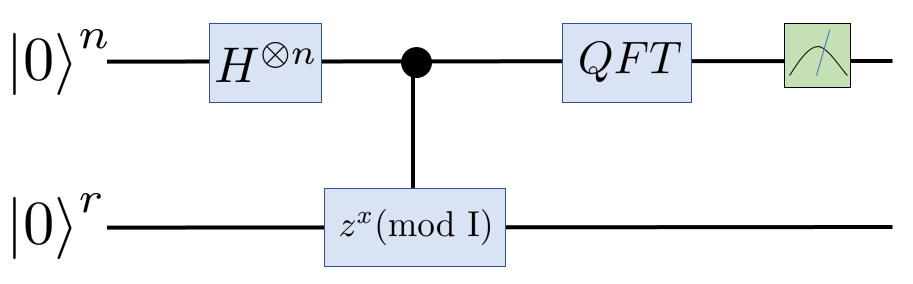
\includegraphics[scale=0.5]{figures/Shor_period_algorithm_circuit.PNG}
 \caption{Circuit diagram for Shor's period finding subroutine}
 \label{fig: period_finding_circuit}
\end{figure}
\subsection{Step 1}
Initialize two quantum registers: input register($\ket{0}^n$ and period register($\ket{0}^r$) where n and r are size of respective registers. Input register stores values of x that are computed to \acrshort{MEF}: $f(x)= z^x$ mod I and period register stores values  for $f(x)$

We determine value of n such that $I^2 \leq 2^n \leq 2I^2$ \cite{loceff2015}, an efficient way is setting $n= \lfloor 2\log I \rfloor$. \cite{chen20007}. Now, since for all z, $x \in \mathbb{Z}_I ^+, I \geq f(x) $, we set $r = \lfloor \log(I) \rfloor + 1 $

We represent the state of the system by
\begin{equation}
    \ket{\Psi_1} = \ket{0}^n \ket{0}^r
\end{equation}

\subsection{Step 2 }
Apply Hadamard gate to 1st register to create a uniform superposition of $N =2^n$ states from 0 to $N-1$. This is initializing the parallelism on the circuit. All the superimposed states serve as inputs for $f(x)$
\begin{equation}
    \ket{\Psi_2} = \frac{1}{\sqrt{N}} \sum_{x=0} ^{N-1} \ket{x}^n \ket{0}^r = \frac{1}{\sqrt{N}} (\ket{0} + \ket{1} + . . . + \ket{N-1}) \ket{0}^r
\end{equation}

\subsection{Step 3}
A random number , $z \in \mathbb{Z}_I ^+ : z \phi I$, is chosen classically. Then the function $f(x) = z^x$ mod I is applied to period register.
\\Here input register is computed to function in the second register. This is achieved by using multiple entangling gates between registers. This step embarks entanglement or co-relation between the two registers.
\\The state of system is represented mathematically as \begin{equation*}
    \ket{\Psi_3} = \frac{1}{\sqrt{N}} \sum_{x=0} ^ {N-1} \ket{x} \ket{f(x)} = \frac{1}{\sqrt{N}} \sum_{x=0} ^ {N-1} \ket{x} \ket{z^x mod I}
\end{equation*}
As discussed in \acrshort{MEF} section \ref{sbsec: MEF}, since $f(x)$ is injective periodic function, we can write $\ket{\Psi_3}$ as 
\begin{equation}
    \ket{\Psi_3} = \frac{1}{\sqrt{N}} \sum_{x=0} ^{a-1} (\sum_{j=0}^{\Tilde{m} - 1} \ket{x + j a}^n ) \ket{f(x)}^r
\end{equation}

\subsection{Step 4}
Now, we perform Conceptual measurement\footnote{Conceptual measurement is a type of measurement that is just done as a mathematical formulation and is usually optional or avoided in practice. It is done for clear understanding of concept or easiness in theoretical study. Also, such measurement does not have any effect on the following circuit} on the period register which collapses the massive superposition into a smaller one. 

We can write \begin{equation*}
    \ket{\Psi_3} = \sqrt{\frac{\Tilde{m}}{N}} \sum_{x=0}^{a-1} (\frac{1}{\sqrt{\Tilde{m}}} \sum_{j=0}^{\Tilde{m} - 1} \ket{x +j a} ) \ket{f(x)}^r
\end{equation*} 

Suppose $\ket{f(x_0)}$ be the output of second register upon measurement. This measurement collapses $x \in {0, 1, 2, . . ., a-1}$ to a single value: $x_0$(say). So, the state become:
\begin{equation*}
    \ket{\Psi_4} = \frac{1}{\sqrt{\Tilde{m}}} \sum_{j=0}^{\Tilde{m} - 1} \ket{x_0 + j a} \ket{f(x_0)}
\end{equation*}
We could ignore $\ket{f(x_0)} $ in the equation as it has no effect on the system. So,
\begin{equation}
    \ket{\Psi_4} =\frac{1}{\sqrt{\Tilde{m}}} \sum_{j=0}^{\Tilde{m} - 1} \ket{x_0 + j a}
\end{equation}



\subsection{Step 5}
Next, we apply quantum Fourier transform on the input register. The state becomes
\begin{equation*}
    \ket{\Psi_5} = QFT \ket{\Psi_4}
    \end{equation*}
\begin{equation*}
                 = \frac{1}{\sqrt{\Tilde{m}}} \sum_{j=0} ^{\Tilde{m} - 1} \frac{1}{\sqrt{N}} ( \sum_{y=0} ^{N-1} w_N ^{(x_0 + j a)y} \ket{y}^n ) 
\end{equation*}
\begin{equation}
    \ket{\Psi_5}   = \frac{1}{\sqrt{\Tilde{m} N}} \sum_{y=0} ^{N-1} w_N ^{x_0 y} \sum_{j=0} ^ {\Tilde{m} - 1} w_N ^{j a y} \ket{y}^n 
    \label{eq: post_QFT}
    \end{equation}
Since second register has been measured(conceptually), $\tilde{m}$ is definite.
Let us define two cases to analyze post QFT remains.
\begin{enumerate}
 \item $\tilde{m}a =  ma = N$
 \item $ma \neq N$
\end{enumerate}
\subsubsection{Case I}
Case II is observed less frequently than the case I. \ref{tab: caseII}
\\When $ ma = N$, we have.
\\$w_N ^{j a y} = e^{\frac{2 \pi j a y}{N}} = e^{\frac{2 \pi i j y}{N}} = w_{m} ^{j y}$
\\and, $\sum_{j=0}^{ \tilde{m}-1} w_N ^{j a y} = \sum_{j=0}^{\tilde{m} -1} w_{m}^{j y} =
\begin{cases}
m & \text{ if $y = 0(mod I)$}\\
0  & \text{if $y \neq 0(mod I)$}
\end{cases}
$
\\Hence equation(\ref{eq: post_QFT}) becomes 
\begin{equation*}
   \ket{\Psi_5} = \frac{1}{\sqrt{mN}} \sum_{y=0}^{N-1} w_N ^{x_0 y} m \ket{y} = \sqrt{\frac{m}{N}} \sum_{y=0}^{N-1} w_N^{x_0 y} \ket{y}
\end{equation*}
Since $y=0$(mod m), $y=cm$ for $c=0, 1, 2, . . .(a-1)$
\begin{equation}
   \ket{\Psi_5} = \frac{1}{\sqrt{a}} \sum_{c=0}^{a-1} w_N^{x_0 c m} \ket{cm}^n
    \label{eq: post_QFT_caseI}
\end{equation}
\subsubsection{Case II}
We are usually more likely to see case II. It can be considered as the general case and hence, the state is given by the equation(\ref{eq: post_QFT}).

\subsection{Step 6: Measurement} \label{sub: step6}
Now, we measure the post-QFT state to obtain the desired output. Upon measurement, let $C=\{y_c\}_{c=0}^{a-1}$ be the set of output measured with high probability. The goal is to determine periodic frequency $m$ so that we can compute period $a= \frac{N}{m}$

For Case I, the state $\ket{\Psi_5}$ \ref{eq: post_QFT_caseI} collapses to set $\{cm\}_{c=0}^{a-1}$ upon measurement. Hence, for case I,  $C=\{y_c\}_{c=0}^{a-1} = \{cm\}_{c=0}^{a-1}$. From this, it seems easy to determine m. But only those $\{cm\}$'s for which c and a are co-prime to each other($c \phi a$) gives nontrivial output. Using Theorem(\ref{th: Riemann_Zeta_function}) we know that there is more than $60\%$ chance that c obtained at random from set $[0,a-1]$ and $a$ are co-prime, i.e. $P(c \phi a) \geq \frac{1}{2}$
\begin{figure}[H]
  \centering
  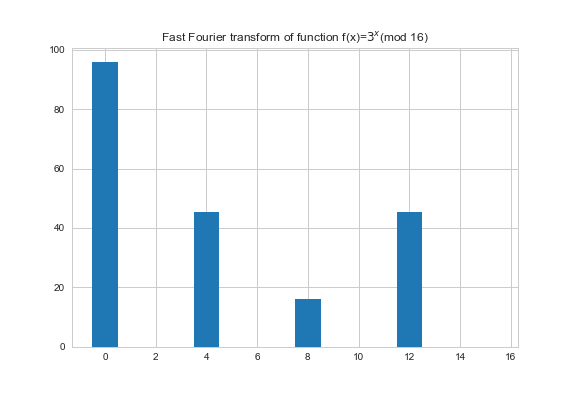
\includegraphics[scale=0.6]{figures/fft_on_3^xmod16.png}
  \caption{Histogram representing discrete Fourier transform on example: \ref{tab: caseI}}
  \label{fig: fft_on_3^xmod16}
\end{figure}

Hence, it is assured that a nontrivial output is obtained more than half the time. Then we obtain the periodic frequency m by applying the Euclidean algorithm on the set of the non-trivial $\{cm\}$'s. 

Analysis of Case II on measurement is more complex than Case I because the state$\ket{\Psi_5}$ (\ref{eq: post_QFT}) does not have an integer frequency: $\frac{N}{a}$ as period a does not divide N exactly. Consider the example \ref{fig: MEF periodic output graph}(b), we can see the function does not complete its full cycle at N. Discrete Fourier transform on the data is shown in the figure(\ref{fig: fft_on_2^xmod15}). It shows multiple points with higher probabilities but does not seems to be multiple of any integer like for case I. 
\begin{figure}[H]
  \centering
  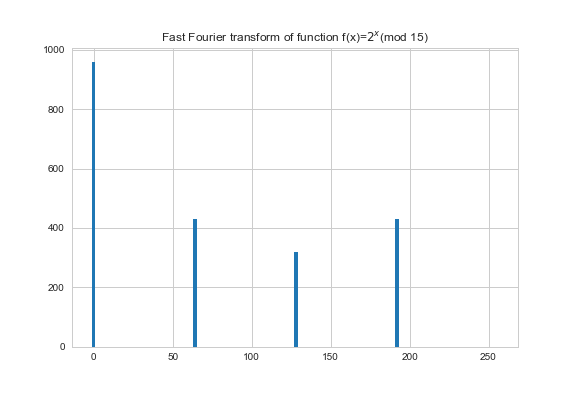
\includegraphics[scale=0.6]{figures/fft_on_2^xmod15.png}
  \caption{Histogram representing discrete Fourier transform on example: \ref{tab: caseII}}
  \label{fig: fft_on_2^xmod15}
\end{figure}

Let us redefine the set $C=\{y_c\}_{c=0}^{a-1}$ for Case II as 
\begin{equation}
    a y_c \in [cN -\frac{a}{2}, cN + \frac{a}{2}]
    \label{eq: yc_limit}
\end{equation}
\begin{equation}
    -\frac{a}{2} \leq a y_c-cN < \frac{a}{2} \Rightarrow |\frac{y_c}{N} -\frac{c}{a}| \leq \frac{1}{2N}
    \label{eq: yc_cont_limit}
\end{equation}
\begin{equation}
    -\frac{a}{2} \leq \hat{y_c} < \frac{a}{2} \text{ where } \hat{y_c} =a y_c-cN
    \label{eq: yc_hat_limit}
\end{equation}
The set $C=\{y_c\}_{c=0}^{a-1}$ is the set of outputs with maximum likelihood upon measurement. The condition above is applied so that the each $y_c$ is expected to converge to $\{cm\}_{c=0}^{a-1}$. We will discuss the relevance of the condition \ref{eq: yc_limit} in the probability section that the set C is the set with maximum likelihood.

\subsection{Step: 7} \label{sub: step7}
We have measured outputs from the quantum computers and now, we analyze the outputs in a classical computer. We use continued fraction algorithm(CFA) and Euclidean Algorithm(EA) on output set $C=\{y_c\}_{c=0}^{a-1}$ to get the period: a. 
\begin{lemma}
    From the set $\{y_c\}_{c=0}^{a-1}$, $\frac{c}{a}$ is in the nearest neighbourhood of $\frac{y_c}{N}$ for any $0<c<a-1$.
    \label{th: nearest_c/a_yc}
\end{lemma}
\begin{proof}
    We know,\begin{equation*}
        \abs{\frac{c+1}{a} -\frac{c}{a}} = \abs{\frac{\pm 1}{a}} \geq \frac{1}{a^2} > \frac{1}{I^2}
    \end{equation*}
    Also we have, $I^2<N$ and from equation \ref{eq: yc_limit},
    \begin{equation}
        \abs{\frac{y_c}{N} -\frac{c}{a}} \leq \frac{1}{2N} \leq \frac{1}{2I^2} \leq \frac{1}{I^2}
        \label{eq: CFA_diff_leq}
    \end{equation}
    So, it is clearly seen that $\frac{c}{a}$ is in vicinity of $\frac{y_c}{N}$ around $\frac{1}{I^2}$, while $\frac{c+1}{a}$ lie outside the vicinity. This proves that "$\frac{c}{a}$ is uniquely close to $\frac{y_c}{N}$."(Loceff, 2015)\cite{loceff2015}
\end{proof}

Let $R= \frac{y_c}{N}$ and since $a<N$, from equation \ref{eq: CFA_diff_leq},
\begin{equation*}
    \abs{\frac{y_c}{N} -\frac{c}{a}} \leq \frac{1}{2I^2}
\end{equation*}
\begin{equation}
    \abs{R -\frac{c}{a}} \leq \frac{1}{2I^2} \leq \frac{1}{2a^2}
    \label{eq: CFA_diff_leq_a2 }
\end{equation}

From lemma(\ref{th: approx_cont_frac}), $\frac{c}{a}$ lies on the convergent sequence of continued fraction for $\frac{y_c}{N}$, given c and a are relatively prime to each other. We will discuss there is a decent probability that c and a are relatively prime later in the study. Since, lemma(\ref{th: nearest_c/a_yc}) suggests $\frac{c}{a}$ is uniquely close to $\frac{y_c}{N}$,  we apply continued fraction algorithm \ref{algo: Continued_fraction_Alorithm} on a set $R= \frac{y_c}{N}$ with error $\frac{a}{2I^2}$.


\begin{conj}
    Continued fraction Algorithm on $\frac{y_c}{N}$ with error $\frac{a}{2I^2}$ outputs unique $\frac{c}{a}$.
\end{conj}
\begin{proof}
    Since $\frac{c}{a}$ is convergent of $\frac{y_c}{N}$ and within the neighbourhood of $\frac{1}{2I^2}$, the output of CFA would be an convergent $\frac{n_k}{d_k} \leq \frac{c}{a}$.
    
    If CFA outputs a convergent: $\frac{n_k}{d_k} <\frac{c}{a}$, it means,
    \begin{equation*}
        \abs{R -\frac{n_k}{d_k}} \leq \frac{1}{2I^2}
    \end{equation*}
    \\But, $d_k$ is strictly increasing according to the properties of convergent of continued fraction and error limit is $E<\frac{1}{2I^2}$.
    \\We have, equation(\ref{eq: CFA_diff_leq_a2 }): \begin{equation*}
        \abs{R -\frac{c}{a}} \leq \frac{1}{2I^2}
    \end{equation*}
    $\frac{c}{a}$ exactly fits the condition. Hence, $\frac{c}{a}$ must be the output of the Algorithm. 
\end{proof}
Since CFA has complexity $O(log^3N)$, We computed an set $\frac{c}{a}$ from $\{y_c\}_{c=0}^{a-1}$ with $O(log^3N)$ complexity. But only those $\frac{c}{a}$ produces nontrivial output for which $c$ and $a$ are co-prime to each other.

Now, we apply Euclidean algorithm on such set $\frac{c}{a}\rfloor_{(c \phi a)}$ to get a value $\frac{1}{a}$. Reciprocal of the value gives the period of the function $f(x)$.

\subsection{Step 8 and 9}
We would check if the calculated period: a is correct. If it is wrong, we would rerun the algorithm for different random $z$. There is a bounded probability that a correct period would be found.

Then, we  would determine the factors classically by applying Euclidean Algorithm: $GCD(z^\frac{a}{2} + 1, N)$ and $GCD(z^\frac{a}{2} - 1, N)$

\section{Probability of Success} \label{probab of success}
We have discussed the steps to determine the factors of a number. But we have introduced the likelihood of happening of certain events. Also, the probabilistic nature of quantum computers causes the result to be expressed in terms of probability. So, as we have discussed, it is not certain that we always obtain the factors. In this section, we will discuss the probabilities involved in the steps during the implementation.

We could enlist the areas for involvement of probabilities as:
\begin{enumerate}
    \item Selection of $z$ co-prime with I
    \item Measurement of $y_c$'s satisfying condition(\ref{eq: yc_cont_limit})
    \item Measurement of $y_c$'s with $c$ co-prime to $a$
\end{enumerate}
\subsection{Measurement of $y_c$'s satisfying condition(\ref{eq: yc_cont_limit})} \label{sub: prob_2}
From step 6, it is evident that for case I: $ma=N$, we obtain each $y_c$ with probability $\frac{1}{a}$. Hence, there is a high likelihood of measuring $y_c$ for case I. 

For case II, we have stated earlier that there is a high likelihood that we obtain $y_c$'s among other $y$ upon measuring the input register. We will prove the statement is true and discuss its relevance.

From step 7, we have equation (\ref{eq: post_QFT}):
\begin{equation}
    \ket{\Psi_5}   = \frac{1}{\sqrt{\Tilde{m} N}} \sum_{y=0} ^{N-1} w_N ^{x_0 y} \sum_{j=0} ^ {\Tilde{m} - 1} w_N ^{j a y} \ket{y}^n 
\end{equation}
Upon measurement, the probability for measuring $\ket{y}$ is 
\begin{equation*}
       P(y) = \abs{\frac{1}{\sqrt{\tilde{m}N}} w_N^{x_0 y} \sum_{j=0}^{\tilde{m}-1} w_N ^{j a y} }^2
\end{equation*}
Here, $\sum_{j=0}^{\tilde{m}-1} w_N ^{j a y}$ is a geometric series,
\begin{equation*}
    \sum_{j=0}^{\tilde{m}-1} w_N ^{j a y} = \abs{\frac{1-(w_N ^{j a y})^{\tilde{m}}}{1-w_N ^{j a y}}} =  \abs{\frac{1-e ^{\frac{2 \pi i a y \tilde{m}}{N}}}{1-e ^{\frac{2 \pi i a y}{N}}  }}
\end{equation*}
The probability of measuring $y_c$ satisfying equation (\ref{eq: yc_cont_limit}) is 
\begin{equation*}
    P(y_c)= \frac{1}{\tilde{m}N}\abs{\frac{1-e ^{\frac{2 \pi i a y_c \tilde{m}}{N}}}{1-e ^{\frac{2 \pi i a y_c}{N}}}}^2
\end{equation*}
Also from \ref{eq: yc_hat_limit}, $\hat{y_c} =a y_c-cN$. Expressing the above equation in-term of $\hat{y_c}$:
\begin{equation}
    P(y_c)= \frac{1}{\tilde{m}N}\abs{\frac{1-e ^{\frac{2 \pi i \hat{y_c} \tilde{m}}{N}}}{1-e ^{\frac{2 \pi i  \hat{y_c}}{N}}}}^2 = \frac{1}{\tilde{m}N}\abs{\frac{1-e ^{i\alpha \tilde{m}}}{1-e ^{i\alpha }}}^2\because \alpha = \frac{2 \pi i \hat{y_c}}{N}
    \label{eq: probability_y_c}
\end{equation}
Since $y_c$'s are the outputs that have a high significance in our problem,  our objective is to determine the lower bound of $P(y_c)$ so that it is explicit for how many times the quantum circuit needs to be executed before getting the required result. For that, we determine the lower bound of the numerator and upper bound of the denominator in $P(y_c)$.

From Euler's identity, we have,
$$1-e^{i\phi} = 1-(cos\phi + i sin\phi)$$
$$= 2 sin\frac{\phi}{2}(cos\frac{\phi}{2} -i sin\frac{\phi}{2})$$
$$\Rightarrow \abs{1-e^{i\phi}}= \abs{2 sin\frac{\phi}{2}}$$

\subsubsection{Upper Bound for denominator}
We know, $\abs{sin \phi} \leq \abs{\phi}$. This statement can be clearly visualized graphically by the figure \ref{fig: sinx_less_than_x}. We can clearly see the line $y=\abs{\phi}$ is clearly above curve $y= \abs{sin \phi} $
\begin{figure}[H]
    \centering
    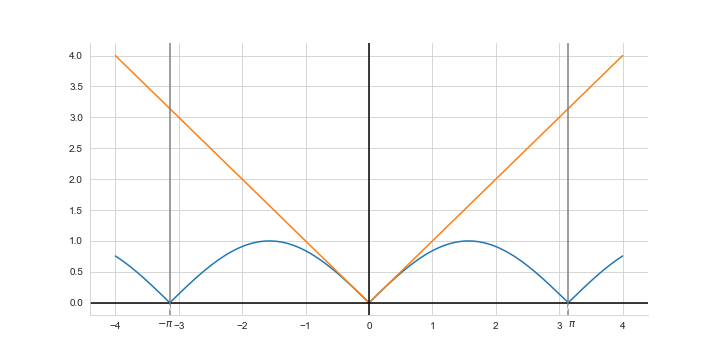
\includegraphics[scale=0.4]{figures/sinx_less_than_x.png}
    \caption{Graph of curves $\abs{sin \phi}$ and $\abs{\phi}$}
    \label{fig: sinx_less_than_x}
\end{figure}
Hence, $$\abs{1-e^{i\alpha}}= 2\abs{sin\frac{\alpha}{2}} \leq \abs{\alpha}$$
The upper bound of the denominator is $\abs{\alpha}$.

\subsubsection{Lower bound of numerator}
The numerator of the fraction has a term $\tilde{m}$ on it whose value is could be $m$ or $m+1$ but distinct. We need to define the lower bound for each case and determine the lowest.

\paragraph{(a). $\tilde{m}=m$\\}
We intend to find the lower bound of term $\abs{1-e^{i\alpha \tilde{m}}} = 2\abs{sin\frac{\alpha}{2}} $
\\ From the definition of $\hat{y_c}$(\ref{eq: yc_hat_limit}), we have,
$$-\frac{a}{2} < \hat{y_c} < \frac{a}{2}$$
$$\Rightarrow -\frac{\pi a m}{N} < \frac{2\pi a m\hat{y_c}}{N} < \frac{\pi a m}{N} $$
        
Since $\frac{am}{N} < 1$,  $-\frac{\pi a m}{N} < -\pi< \frac{2\pi a m\hat{y_c}}{N} < \frac{\pi a m}{N} < \pi$
        
$$\Rightarrow -\pi< \frac{2\pi a m\hat{y_c}}{N}=\alpha m <  \pi$$
\begin{figure}[H]
    \centering
     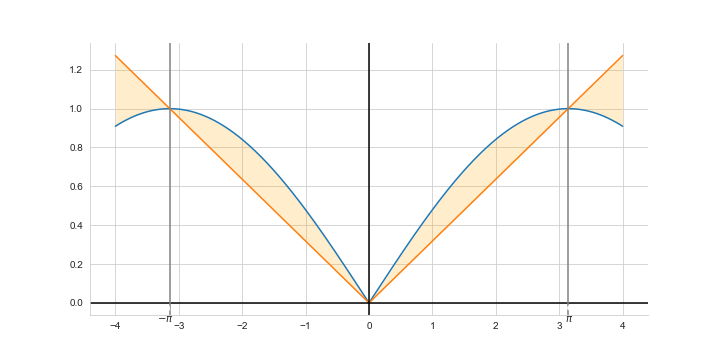
\includegraphics[scale=0.4]{figures/sinx__2_less_than_x__pi.png}
    \caption{Graph of curves $\abs{sin\frac{\phi}{2} }$ and $\abs{\frac{\phi}{\pi}} $}
    \label{fig: sinx__2_less_than_x__pi}
\end{figure}
The graph on the figure (\ref{fig: sinx__2_less_than_x__pi} shows the plot of curve $y= \abs{sin\frac{\phi}{2}}$ and a line $y= \abs{\frac{\phi}{\pi}} $. For a limit $-\pi < \phi< \pi$, the graph shows $\abs{sin\frac{\phi}{2}} > \abs{\frac{\phi}{\pi}} $.
So, the lower bound of $\abs{a-e^{i\phi}}$ in interval $[-\pi/2, \pi/2]$ is $\abs{\frac{\phi}{\pi}}$
\\Hence, we can write,
$$\abs{1-e^{i\alpha m}} = 2\abs{sin\frac{\alpha m}{2}} \geq 2\abs{\frac{\alpha m}{\pi}} $$  

        
It can also be proven analytically using calculus.

Then, the minimum likelihood of obtaining $y_c$ using equation(\ref{eq: probability_y_c}): 
$$ P(y_c)_{\tilde{m}=m} = \frac{1}{mN}\abs{\frac{1-e ^{i\alpha \tilde{m}}}{1-e ^{i\alpha }}}^2 > \frac{1}{mN} \abs{\frac{2\abs{\frac{\alpha m}{\pi}}}{\abs{\alpha}}}^2$$
\begin{equation}
    P(y_c)_{\tilde{m}=m} \leq \frac{4m}{ \pi^2 N}
    \label{eq: probability_yc_m}
\end{equation}

\paragraph{(b). $\tilde{m} = m+1$\\}
For this sub-case, we follow the same steps with some minor changes. We had,
$$-\frac{a}{2} < \hat{y_c} < \frac{a}{2}$$
$$\Rightarrow -\frac{\pi a (m+1)}{N} < \frac{2\pi a m\hat{y_c}}{N} < \frac{\pi a (m+1)}{N} $$
        
Since $\frac{a(m+1)}{N} < 1$ and $\frac{a}{N} < \frac{1}{2}$,  $$-\frac{\pi a (m+1)}{N} < \frac{-3\pi}{2}< \frac{2\pi a (m+1)\hat{y_c}}{N} < \frac{\pi a (m+1)}{N} < \frac{3\pi}{2}$$
        
$$\Rightarrow \frac{-3\pi}{2}< \frac{2\pi a (m+1)\hat{y_c}}{N}=\alpha (m+1)<  \frac{3\pi}{2}$$
\begin{figure}[H]
    \centering
     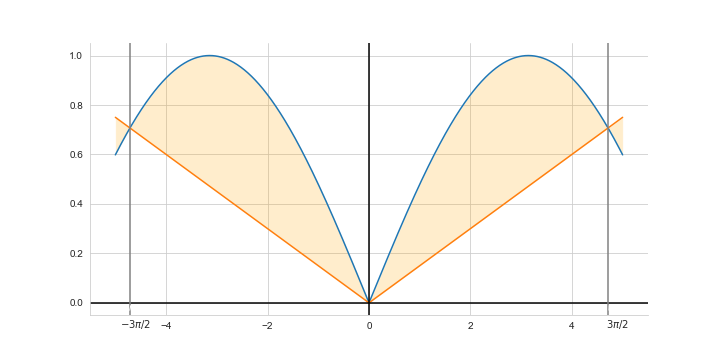
\includegraphics[scale=0.4]{figures/sinx__2_less_than_k_x__pi.png}
    \caption{Graph of curves $\abs{sin\frac{\phi}{2} }$ and $\abs{k\frac{\phi}{\pi}} $, $k= \frac{2}{3} sin\frac{3\pi}{4}$}
    \label{fig: sinx__2_less_than_k_x__pi}
\end{figure}
Here,in the graph, curve $\abs{sin\frac{\phi}{2} }$ exactly bound a line $\abs{\frac{k\phi}{\pi}}$ where $k= \frac{2}{3} sin\frac{3\pi}{4}$  in the interval $[-3\pi/2,3\pi/2]$. In contrast to the previous sub-case, a constant k is multiplied to the term $\abs{\frac{\phi}{\pi}}$ for balancing. We can clearly state $\abs{sin\frac{\phi}{2}} > \abs{k\frac{\phi}{\pi}}$ where $k= \frac{2}{3} sin\frac{3\pi}{4}$. So, the lower bound of $\abs{1-e^{i\alpha (m+1)}}$ in interval $[-3\pi/2, 3\pi/2]$ is $\abs{k \frac{\alpha (m+1)}{\pi}}$
\\Hence, the minimum likelihood of obtaining $y_c$ is
$$ P(y_c)_{\tilde{m}=m+1} = \frac{1}{(m+1)N}\abs{\frac{1-e ^{i\alpha (m+1)}}{1-e ^{i\alpha }}}^2 > \frac{1}{(m+1)N} \abs{\frac{2\abs{\frac{k^2\alpha (m+1) k^2}{\pi}}}{\abs{\alpha}}}^2$$
\begin{equation}
    P(y_c)_{\tilde{m}=(m+1)} \geq \frac{(4 (m+1) k^2)}{\pi^2 N}
    \label{eq: probability_yc_m+1}
\end{equation}

We can generalize the minimum likelihood of measuring $y_c$ for cases $\tilde{m}=m$ or $m+1$ as 
\begin{equation}
    P(y_c)_{\tilde{m}} \geq \frac{4 \tilde{m} k^2}{\pi^2 N}
    \label{eq: probability_yc_general}
\end{equation}
But there are 'a' numb such $\{y_c\}$'s obtained after measurement: $y_1,y_2,\dots ,y_{a-1}$. So minimum probability of measuring any one of the $\{y_c\}'s$ is 
\begin{equation}
    P(y_c)_{\tilde{m}} \geq \frac{(4 a\tilde{m} k^2)}{\pi^2 N}
    \label{eq: probability_one_yc_general}
\end{equation}

Let us study the worst-case scenario in obtaining any one of $\{y_c\}'s$. We have assumed a condition: $2a<N$ earlier in the study. The worst-case for the minimum likelihood of measuring $y_c$ is when $3a>N$. For minimum case, this implies $\frac{am}{N}>\frac{1}{2}$ and $\frac{a(m+1)}{N}>1$
\begin{equation*}
    P(y_c)_{\tilde{m}} \geq \frac{4 k^2}{\pi^2 }\frac{a(m+1)}{N}>\frac{4 k^2}{\pi^2}= 0.090
\end{equation*}
But typically, we have $a<<I<N$, so $\frac{a\tilde{m}k^2}{N} \equiv 1$. Then the inequality becomes:
\begin{equation*}
    P(y_c)_{\tilde{m}} \geq \frac{4 k^2}{\pi^2 }\frac{a\tilde{m}}{N}>\frac{4}{\pi^2}=0.405 
\end{equation*}
Hence, the probability of measuring any one of $\{y_c\}'s$ is 
\begin{equation*}
P(y_c)^{min}=
    \begin{cases}
        0.090 &\text{For worst case}\\
        0.405 &\text{typically}
    \end{cases}
\end{equation*}

Now, let us compute the maximum likelihood of obtaining $y_c$.
The upper bound of the numerator could be easily determined using the relations defined above.
We know, $$\abs{a=e^{i\alpha \tilde{m}}} = 2sin(\frac{\alpha}{2}) \leq \alpha \tilde{m} $$
However, we need to determine new limit for the lower bound of denominator. We have, 
$$-\frac{a}{2} < \hat{y_c} < \frac{a}{2}$$
$$\Rightarrow -\frac{\pi a}{N} < \frac{2\pi a \hat{y_c}}{N} < \frac{\pi a}{N} $$
        
Since $\frac{a}{N} < \frac{1}{2}$,  $$-\frac{\pi a}{N} < \frac{\pi}{2}< \frac{2\pi a \hat{y_c}}{N} < \frac{\pi a}{N} < \frac{\pi}{2}$$
        
$$\Rightarrow \frac{\pi}{2}< \alpha <  \frac{\pi}{2}$$
\begin{figure}[H]
    \centering
     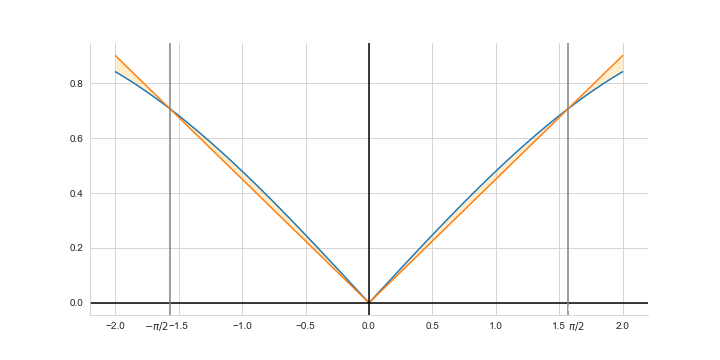
\includegraphics[scale=0.4]{figures/sinx__2_less_than_l_x__pi.png}
    \caption{Graph of curves $\abs{sin\frac{\phi}{2} }$ and $\abs{k\frac{\phi}{\pi}} $, $k= 2 sin\frac{\pi}{4}$}
    \label{fig: sinx__2_less_than_l_x__pi}
\end{figure}
Here, in the graph, curve $\abs{sin\frac{\phi}{2} }$ exactly bound a line $\abs{\frac{l\phi}{\pi}}$ where $l= 2 sin\frac{\pi}{4}$  in the interval $[-\pi/2,\pi/2]$. In contrast to the previous sub-case, a constant k is multiplied to the term $\abs{\frac{\phi}{\pi}}$ for balancing. We can clearly state $\abs{sin\frac{\phi}{2}} > \abs{l\frac{\phi}{\pi}}$ where $l= 2 sin\frac{3\pi}{4}$. So, the lower bound of $\abs{1-e^{i\alpha}}$ in interval $[-\pi/2, \pi/2]$ is $\abs{l\frac{\alpha}{\pi}}$.
\\Hence, the maximum likelihood for obtaining $y_c$ is 
$$P(y_c)^{max} \leq \frac{1}{\tilde{m}N}\abs{\frac{2\alpha \tilde{m} }{\pi l\alpha}}^2 =\frac{4(m+1)}{\pi^2 l^2 N}$$,$\tilde{m}=m+1$ for maximum likelihood.

Now, as a metric of the likelihood for not measuring $y_c$, we determine the ratio of minimum and the maximum likelihood of $y_c$ as
\begin{equation}
   \mathcal{P}_{ratio} = \frac{P(y_c)^{min}}{P(y_c)^{max}} \geq \frac{\frac{4m k^2}{ \pi^2 N}}{\frac{4(m+1)l^2}{\pi^2  N}} = \frac{m}{m+1}\frac{k^2}{l^2} \geq \frac{2}{3}\frac{k^2}{l^2} 
\end{equation}
We know,for large $I$ and N, $\frac{m}{m+1} \approx 1$ and  $k,l \approx 1$. So, $\mathcal{P}_{ratio}$ can be expressed as:
\begin{equation*}
    \mathcal{P}_{ratio} >
    \begin{cases}
        0.72 &\text{worst case}\\
        1-\epsilon &\text{otherwise}
    \end{cases}
\end{equation*}
$\epsilon$ is the error limit.
\subsection{Measurement of $y_c$'s with $c$ co-prime to $a$}
We measure ${y_c}$'s with a certain high probability upon a set of measurement. We have described that we use continued fraction algorithm on the set ${\frac{y_c}{N}}$ to determine a set ${\frac{c}{a}}$. But out of this set $\frac{c}{a}$, only these elements that satisfy condition $c \phi a$, i.e c and a are co-prime, are non-trivial. In this subjection, we will discuss the probability of randomly selected c to satisfy the condition $c \phi a$.

We can say, the probability $P(c \phi a)$ is the probability that there is no common prime factor of a and c.
$P(c \phi a) = P$(no common factor between a and c)
Let ${2, 3, 5, 7, . . . p_k}$ be the set of prime numbers less than a, then,
\\$P(c \phi a) = P(\neg (2 \mid c \wedge 2 \mid a) \wedge (3 \mid c \wedge 3 \mid a) . . . \wedge (p_k \mid c \wedge p_k \mid a)) $\\
    $$= \Pi_{p_i =primes}^{p_k < a} P(\neg (p_i \mid c \wedge p_i \mid a))$$ 
\\And we know, $P(p \mid c ) < \frac{1}{p}$ and $P(p \mid a) < \frac{1}{p}$
\\Then $P(\neg (p \mid c) \wedge (p \mid a)) \geq 1 - \frac{1}{p^2} $
\\Hence, $P(c \phi a) > \Pi_{p_i =primes}^{p_k < a} (1 - \frac{1}{p^2})$
\\This looks similar to the Riemann Zeta function in Euler's product form.
\\Riemann Zeta function is a special type of Dirichlet series analytic in domain in complex plane c given by $\zeta(s) = \sum_{n=1}^\infty \frac{1}{n^s}$ ,where Real part of s, $Re(s)>1$. The function converges when $Re(s) >1 $.
\\A special case of Riemann zeta function as $s=2$ is of interest to us.
\\$$\zeta(1) = \frac{\pi^2}{6} = \sum_{n=1}^\infty = 1 + \frac{1}{2^2} + \frac{1}{3^2} + . . .$$
\\It is a very popular identity of Pi and can be proved (Appendix) easily.
\begin{lemma}
    Riemann Zeta function, $\zeta(s) = \sum_{n=1}^\infty \frac{1}{n^s}$, $Re(s) > 0$ can be written in form
    $$\zeta(s) = \Pi_{n=1}^\infty \frac{1}{1-\frac{1}{p_n^s}} $$ where ${p_n}$ is the sequence of all the primes.
    \label{th: Riemann_Zeta_function}
\end{lemma}
Using Theorem (\ref{th: Riemann_Zeta_function})
$$\Pi_{n=1}^\infty (1-\frac{1}{p^2}) = \frac{1}{\zeta(2) = \frac{6}{\pi^2}}$$
$$P(c \phi a) > \frac{6}{\pi^2 } \approx 0.607$$
Thus there is $60\%$ likelihood that we obtain non-trivial function ${\frac{c}{a}}$.
\subsection{Finalizing Probability}
In this subsection, we shall integrate all the probability to see the probability of success of the algorithm. 
\\We have, the set of high probability measurements $c={y_c}_{c=0}^{a=1}$. Let us define a new set
$$B= {y_p : y_p \in C \wedge (b \phi a)  }$$
$$B \leq C$$
Let $\abs{C}$ and $\abs{B}$ be the size of each set C and B respectively.
\\The ratio of size of the sets $\frac{\abs{B}}{\abs{C}}$ gives the probability of $P(b \phi a)$.
So, $$ \frac{\abs{B}}{\abs{C}} = P(b \phi a) > 0.607$$

Here our goal is to determine probability of obtaining the set B i.e $P(B)$
$$P(B) = P(B \mid C) . P(C)$$
$$= \frac{\sum_{b \in B} P(y_b)}{\sum_{c \in C} P(y_c)} . P(y_c)$$

Let $P(y_b^{min})$ and $P(y_c^{max})$ be minimum likelihood of obtaining $y_b$ and maximum likelihood of obtaining $y_c$. 
\\Then, $P(B) > \frac{\abs{B}}{\abs{C}} \frac{P(y_b^{min})}{P(y_c^{max})} . P(y_c)$

For worst case, $P(B) > 0.607 \times 0.72 \times 0.405 (\frac{6}{\pi^2} \times 0.72 \times \frac{4k^2}{\pi^2})$
$\approx 0.177$
\\For typical case, $P(B) > 0.607 \times 1 \times 0.405$
$\approx 0.246$

Hence, the probability of failure in this algorithm is bounded. Shor's algorithm is called the bounded error algorithm for this reason.

\paragraph{}
A constant time algorithm is an algorithm that completes after a fixed number of trials of loops, T where T is independent of the size of the algorithm N

\begin{theorem}[Constant Time Complexity theorem(CTC theorem)]
    If a probabilistic, looping algorithm having size N, has a bounded non-zero probability of success for a single loop, independent of N, then it is a constant time algorithm. \cite{loceff2015}(loceff, 2015)
    \\$P(success) = p>0$, p is independent of N
    \label{th: Constant_Time_Complexity_theorem}
\end{theorem}

We can see, this period finding subroutine of Shor's algorithm satisfies the necessary condition of the CTC theorem(\ref{th: Constant_Time_Complexity_theorem}). So, it is a constant time algorithm. The number of trials for a constant time algorithm with error tolerance $\epsilon$ and probability of success of single-trial p is given by:
\begin{equation*}
    T = \left \lfloor \frac{log(\epsilon)}{log(1-p)} \right\rfloor  + 1
\end{equation*}
Thus, the period finding subroutine for a certain 'z' is likely to output period 'a' in
\begin{equation*}
    T = \left \lfloor \frac{log(\epsilon)}{log(1- P(B)} \right\rfloor  + 1
\end{equation*}
\section{Complexity of Algorithm}
Now let us discuss the complexity of the algorithm. We can divide the algorithm into 5 parts: Hadamard gates, QFT, oracle operation for $f(x)$, CFA (continued fraction algorithm), and other classical subroutines.
\\We have computed most of the section of the algorithm on the n qubit system. So, the complexity obtained will be expressed in terms of $N$ or $n$. We aim to express the complexity in terms of the integer I. 
\\ We have, $$\frac{N}{2}\leq I^2 \leq N$$
$$log(N)-log(2)\leq 2log(I) \leq log N $$ 
$$\Rightarrow \mathcal{O}(log(N)) \leq \mathcal{O}(I)\leq \mathcal{O}$$
Hence, $\mathcal{O}(N)=\mathcal{O}(I)$ is the relation between the Big $\mathcal{O}$ operation on I and N. Further on, we will replace $\mathcal{O}(N)$ by $\mathcal{O}(I)$ for consistency and generalization.


The complexity of Hadamard gates on n qubits is $\mathcal{O}(log(N)) = \mathcal{O}(log(I))$ and QFT is $\mathcal{O}(log^2(I))$. We had discussed CFA has complexity of $\mathcal{O}(log^3(I))$ . Other classical operations include obtaining GCD whose complexity is less than $\mathcal{O}(log^3(I))$. So they can be ignored during complexity computation. Determination of complexity of oracle operation needs thorough analysis of the function f(x).

The complexity for oracle operation of function $f(x)$ is same as the complexity for determining $f(x)$.
\\ We have, $$f(x)=z^x mod I$$
We need to compute the term $z^x$. let us express x n binary form as $x= \sum_k x_k 2^k$. Since, $x<n$, we can write $x= \sum_{k=0}^{n-1} x_k 2^k$. So,
$$ z^x = z^{\sum_{k=0}^{n-1} x_k 2^k} = \Pi_{k=0}^{n-1} z^{x_k 2^k}  $$
An efficient way to compute the set $ \{2^k\}_{k=0}^{n-1}$ is to perform repeated squaring $z$ till the power is $(n-1)$ as $2^j =(2^{j-1})^2$. This process only requires n-2 steps. Also multiplication by $x_k$ is a decision problem as $x_k= \{0,1\}$ and has constant complexity. Since, each multiplication operation is $\mathcal{O}(log^2(N))$, by adding $\mathcal{O}(log(N))$ operation, we get the set $ \{2^k\}_{k=0}^{n-1}$ by $\mathcal{O}(log^3(N))$ operations. This operation is done classically. 

Now, we use set $ \{2^k\}_{k=0}^{n-1}$ to determine $z^x$ by $n=log(N)$ product operations each of $\mathcal{O}(log^2(N))$ on quantum computer followed by modulo operation. So, the total operations is $\mathcal{O}(log^3(N))$. Hence, oracle operation is  $\mathcal{O}(log^3(I))$.

Thus, the subroutines of Shor's factoring algorithm with their complexity is tabulated as:
\begin{table}
\begin{center}
\begin{tabular}[h!]{|l|l|}
	\hline
	Subroutine & Complexity\\
	\hline
	Hadamard gates	& $\mathcal{O}(log(I))$\\
	QFT		& $\mathcal{O}(log^2(I))$\\
	Oracle function & $\mathcal{O}(log^3(I))$\\
	CFA	 	& $\mathcal{O}(log^3(I))$\\
	Classical operations & $\mathcal{O}(log^3(I))$\\
	\hline
\end{tabular}

 \caption{Complexity of processes in Shor's algorithm}
    \label{tab: Complexity of processes in Shor's algorithm}
\end{center}
\end{table}

Since each subroutine is independent of others, the complexity of the algorithm is $\mathcal{O}(log^3(I))$. Hence we can conclude that Shor's algorithm is a quantum algorithm, capable of factoring integers in polynomial complexity with bounded error probabilities. Thus Shor's algorithm is a \acrshort{BQP}(bounded-error quantum polynomial) algorithm.
